\section{Projeto Elétrico Start X}

Com o intuito de utilizar a energia elétrica convertida a partir da energia mecânica oriunda da pedalada do usuário, torna-se imperioso o dimensionamento de um circuito elétrico de armazenamento e distribuição da referida energia elétrica visando ao uso desta para alimentar as cargas de nosso projeto. Assim, a presente seção abordará o projeto elétrico do projeto em tela.

\subsection{Levantamento das Cargas}
\label{levantamento-cargas}

A primeira etapa para o dimensionamento de um projeto elétrico consiste no levantamento das cargas que serão alimentadas pelo circuito de distribuição de energia elétrica a ser projetado. Nesse sentido, as cargas do presente projeto serão aquelas informadas na Tabela \ref{cargas-dispositivos}.

\begin{table}[h]
\centering
\begin{tabular}{|l|l|}
\hline
\rowcolor[HTML]{329A9D} 
CARGA                                                           & QUANTIDADE \\ \hline
Carregador de Celular & 1          \\ \hline
Sensores                                                        & 7          \\ \hline
\end{tabular}
\caption{Levantamento das cargas do Projeto Elétrico START X.}
\label{cargas-dispositivos}
\end{table}

Continuando, em posse dessas cargas, a próxima etapa consiste em estimar a potência elétrica requerida pelas mesmas. Esse cálculo pode ser realizado conforme Equação \ref{potencia-requerida}

\begin{equation}
	\mathcal{P} = v \times i \times fp
	\label{potencia-requerida}
\end{equation}

Onde:
\begin{description}

\item [P] potência da carga em watt

\item [V] tensão elétrica em volt

\item [I] corrente elétrica em ampère

\item [fp] fator de potência (adimensional)
\end{description}

Ocorre que o carregador de celular listado na Tabela 1 não será produzido por nós, dificultando assim o cálculo exato de sua potência através da Equação 1, devido à existência de diversos modelos fabricados atualmente. Desse modo, usar-se-á modelo já fabricado para essa carga. Conforme relatado a respeito da existência de diversos modelos de carregadores fabricados atualmente, para o levantamento da potência dessa carga, usar-se-á dado de potência utilizado a partir de consulta junto ao sítio eletrônico da Eletrobrás – Distribuição Piauí, cujo valor é utilizado pela referida Distribuidora para fazer a simulação de consumo mensal de residências. Nesse ponto, apresenta-se o valor da supracitada potência (Figura \ref{levantamento-de-potencias}).

% Pegar figuras.
\begin{figure}[h]
	\centering
	%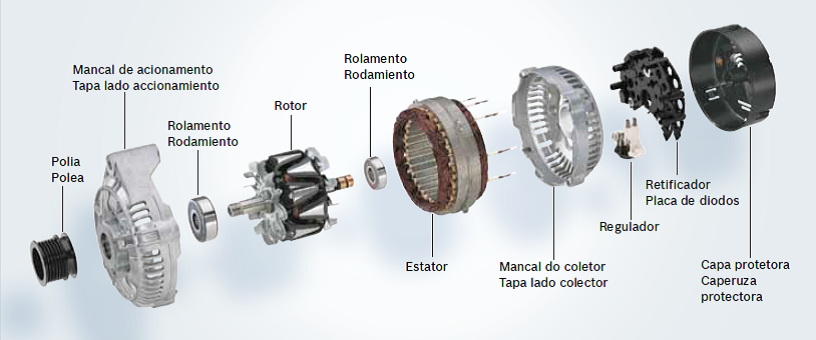
\includegraphics[scale= 0.8]	{figuras/partes_alternador.png}
	\caption{Dado utilizado para o levantamento de potência do carregador de celular a ser utilizado no Projeto Elétrico Start X. Fonte: <  http://www.eletrobraspiaui.com/simulador.php >}
	\label{levantamento-de-potencias}
\end{figure}

Já em relação à potência requerida pelos supracitados sensores, informa-se que foi realizada estimativa junto aos integrantes da Engenharia Eletrônica presentes no presente projeto, no tocante às grandezas elétricas dos referidos sensores, isto é, corrente e tensão elétrica de trabalho; ainda, assumiu-se que o fator de potência dos mesmos é igual a 1, ou seja, tratou-os como cargas resistivas. Assim, os resultados estimados para essas cargas encontram-se dispostos na Tabela \ref{grandezas-eletricas}.

\begin{table}[h]
\centering
\begin{tabular}{|l|l|}
\hline
\rowcolor[HTML]{329A9D} 
GRANDEZA ELÉTRICA & VALOR                                            \\ \hline
Corrente                                                    & 500Ma 
\\ \hline
Tensão                                                      & 5V
\\ \hline
Fator de Potência & 1                                                \\ \hline
\end{tabular}
\caption{Grandezas elétricas dos sensores do Projeto Elétrico Start X.}
\label{grandezas-eletricas}
\end{table}

Assim, em posse das informações da Tabela acima, e utilizando-se a Equação 1, conseguiu-se o valor quantitativo da potência elétrica requerida pelos sensores em comento. Esse valor, bem como o valor estimado para a potência requerida pelo carregador de celular são indicados na Tabela \ref{estimativa-requerida}. 

\begin{table}[h]
\centering
\begin{tabular}{|l|l|}
\hline
\rowcolor[HTML]{329A9D} 
CARGA                                                           & POTÊNCIA                                                   \\ \hline
Carregador de Celular                                           & 15W   
\\ \hline
Sensores                                                        & 2,5W * 7 = 17,5W 
\\ \hline
TOTAL                                                           & 32,5W                                                      \\ \hline
\end{tabular}
\caption{Estimativa da potência requerida pelas cargas do Projeto Elétrico Start X.}
\label{estimativa-requerida}
\end{table}
	
Portanto, o projeto elétrico aqui proposto deverá alimentar cargas que requerem 32,5 watts de potência.

\subsection{Fonte Geradora}
\label{fonte-geradora}

Para que ocorra a conversão eletromecânica de energia no presente projeto, um dos requisitos necessários é a presença de uma fonte geradora de energia elétrica. Nesse passo, após cuidadoso levantamento da potência requerida pelas cargas existentes em nosso projeto, cuidou-se em conseguir a fonte geradora que pudesse atender à exigência de potência solicitada.

Ainda, além de cumprir com a exigência de potência acima mencionada, buscou-se uma fonte que pudesse realizar a integração entre as Engenharias Automotiva e de Energia, a fim de que os integrantes destes cursos pudessem explorar conhecimentos pertinentes ao funcionamento e utilidade da referida fonte.
Pois bem, como resultado, escolheu-se como fonte do presente projeto uma máquina elétrica síncrona exercendo função geradora. Ainda, sendo mais específico, foi escolhido um alternador automotivo (Figura \ref{alternador}).

\begin{figure}[h]
	\centering
	%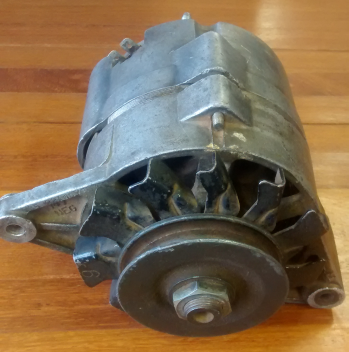
\includegraphics[scale=0.8]		{figuras/alternador.png}
	\caption{Fonte Geradora de Energia Elétrica do Projeto Elétrico Start X: alternador automotivo.}
	\label{alternador}
\end{figure}

A fim de confirmar o atendimento da potência requerida pelas cargas, apresenta-se a seguir, na Tabela \ref{grandezas-alternador}, os valores quantitativos nominais referentes às grandezas elétricas do supracitado alternador.

\begin{table}[h]
\centering
\begin{tabular}{|l|l|}
\hline
\rowcolor[HTML]{329A9D} 
PROPRIEDADE                                                           & VALOR                                                   \\ \hline
Corrente & 35 A 
\\ \hline
Tensão & 14V
\\ \hline
Fator de Potência\protect\footnotemark  & 1                                                      \\ \hline
Potência & 490W
\\ \hline
\end{tabular}
\caption{Grandezas nominais do alternador presente no Projeto Elétrico Start X.}
\label{grandezas-alternador}
\end{table}
\footnotetext{Não foi possível estimar o fator de potência do alternador, por isso, em uma aproximação grosseira, considerou-o igual a 1.}

Analisando-se a Tabela anterior, verifica-se que a potência nominal da fonte escolhida está acima da potência necessária à alimentação das cargas e, por consequência, resta atendido essa necessidade. 
Ainda em sede justificativa da escolha da fonte geradora, especificamente no tocante à integração das engenharias acima citadas, o uso do alternador automotivo no presente projeto permite que ocorra a almejada integração, pois a partir de seu uso no circuito aqui discutido, podem ser explorados conhecimentos relacionados às máquinas síncronas (Engenharia de Energia) e também conhecimentos inerentes a elementos automotivos (Engenharia Automotiva), por exemplo.
Pois bem, uma vez escolhido e justificado os motivos que ocasionaram na determinação da fonte geradora escolhida, passa-se a seguir a abordar a respeito da mesma.

\subsubsection{Alternador: Princípio de Funcionamento}
\label{alternador-funcionamento}


O uso de geradores síncronos é bastante comum em centrais elétricas de grande porte, independente do seu tipo. A propósito, grande parcela da energia elétrica disponível mundialmente, e transmitida/distribuída na rede elétrica é gerada por esses geradores, os quais realizam a conversão da energia mecânica em energia elétrica. 

Ainda, além do uso das centrais geradoras de energia elétrica de grande porte, os geradores síncronos são usados na geração de energia de pequeno porte e também em centrais autônomas, isto é, centrais não conectadas à rede elétrica convencional, como é o caso do presente projeto.

O alternador aqui adotado encontra-se incluído no rol das máquinas síncronas com função geradora. Por oportuno, apresenta-se o conceito do que seja uma máquina síncrona: (FITZGERARD, 2008): “Uma máquina síncrona é uma máquina elétrica cuja rotação é proporcional à frequência da rede à qual está conectada”. Ainda, o nome síncrono se deve ao fato de esta máquina operar com uma velocidade de rotação constante sincronizada com a frequência da tensão elétrica alternada aplicada aos terminais da mesma, ou seja, devido ao movimento igual de rotação entre o campo girante e o rotor (sincronismo entre campo do estator e rotor).

O princípio de funcionamento dos geradores síncronos, dentre eles o alternador, baseia-se na indução eletromagnética, ou seja, a corrente elétrica flui através do rotor criando um campo magnético que induz a movimentação dos elétrons nas bobinas do estator, resultando em uma corrente alternada.

No caso do alternador, no automóvel, ele é acionado pelo motor do veículo no momento da ignição, através de uma correia sincronizadora, sendo o responsável pela produção de energia elétrica que irá alimentar os consumidores elétrico do automóvel. Ao contrário do que muitas pessoas imaginam, é o alternador, e não a bateria, quem alimenta todos os consumidores elétricos durante o funcionamento do veículo. Consequentemente é ele também, o responsável por recarregar a bateria.

 Ocorre que os automóveis operam com corrente contínua e, por isso, há a necessidade de transformar a corrente alternada gerada pelo alternador em contínua. Assim, nos alternadores automotivos existe a adição de dois componentes fundamentais: a placa retificadora (retificador), que transforma a corrente alternada em contínua, e o regulador de tensão, responsável pelo controle da tensão produzida.
Desse modo, constata-se que, enquanto a tensão disponibilizada pelo gerador síncrono clássico utilizado em centrais geradoras é alternada, no alternador automotivo, não obstante a tensão gerada seja alternada, devido ocorrer a retificação e regulação dessa tensão para aproximadamente 12 volts, sendo após isso direcionada à bateria, a tensão de saída do mesmo é contínua. Dada essa peculiaridade constitucional, as demais partes constituintes do alternador são as mesmas do gerador síncrono clássico. Por isso, vejamos. 

\subsubsection{Partes Constituintes}
\label{construtivas-gerador-sincrono}

O alternador é composto de acordo com as partes demonstradas na Figura \ref{partes-alternador}.

\begin{figure}[h]
	\centering
	%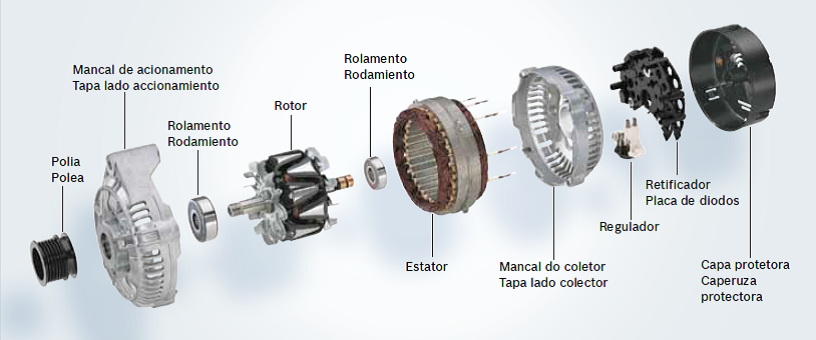
\includegraphics[scale= 0.8]		{figuras/partes_alternador.png}
	\caption{Partes que compõem um alternador. Fonte: Bosch, 2014. }
	\label{partes-alternador}
\end{figure}

Não obstante todos os componentes demonstrados na Figura 3 sejam importantes, para o caso do projeto elétrico aqui discutido, serão abordados comentários a respeito apenas de alguns dos componentes presentes na Figura 3, os quais influenciaram significativamente o desempenho de nosso alternador. Vejamos. 

\begin{description}

\item [Rotor]

O processo de geração da energia elétrica se inicia no rotor. O rotor aborda a parte móvel no centro do alternador, sendo constituído por um eixo de aço envolto por um par de rodas polares, com uma bobina enrolada em seu interior, na qual a quantidade de fios de cobre da bobina varia de acordo com a capacidade e especificações de cada alternador. A Figura \ref{rotor-alternador}, é ilustrado o rotor do alternador utilizado no presente trabalho, representado pelo número 1.

\begin{figure}[h]
	\centering
	%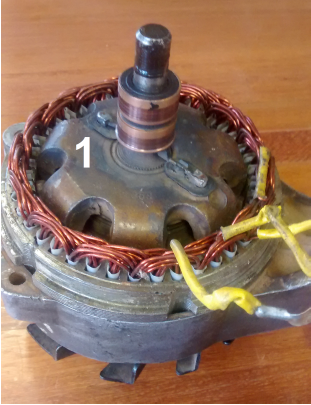
\includegraphics[scale=0.8] {figuras/rotor_alternador.png}
	\caption{Rotor do alternador presente no Projeto Elétrico Start X.}
	\label{rotor-alternador}
\end{figure}

A função principal do rotor consiste em formar um campo magnético que tem como resultado a produção de corrente elétrica, onde os seus polos são alimentados com corrente contínua e, a partir daí, geram o campo principal que induz tensão na armadura (estator).

Para que ocorra a indução do referido campo magnético, e por consequência o início da geração de energia elétrica, é necessário que haja uma corrente de excitação, a qual deve ser conduzida até o enrolamento de campo (rotor), a fim de ser criado o campo magnético já citado. 

A corrente contínua de excitação requerida para a alimentação do enrolamento de excitação do nosso alternador será conduzida até o rotor por meio de escovas condutoras de energia elétrica. 

A literatura informa que a potência contínua requerida para a excitação aproxima-se de 1\% da nominal. Para o nosso projeto, a corrente necessária à excitação ora em comento será fornecida por uma bateria que atenda a capacidade de potência (excitação) requerida.

\item [Estator]

O estator é formado por um conjunto de bobinas isoladas entre si e fixadas em um conjunto de laminas de aço. Essas lâminas têm características magnéticas de alta permeabilidade, proporcionando um caminho com pequena relutância para o fluxo, o que diminui o fluxo disperso e concentra o campo no entreferro. 

O uso de lâminas na construção do estator proporciona a diminuição das perdas provocadas por correntes parasitas em relação ao emprego de uma estrutura maciça. As mencionadas lâminas também são tratas termicamente para diminuir o valor das perdas geradas por correntes induzidas.

A principal função do estator é a geração da corrente elétrica alternada. Entretanto, conforme já informado, para que ocorra a geração de energia elétrica, inicialmente, as bobinas do estator requerem a produção de um campo magnético pelo rotor, sendo este campo magnético potencializado pelas garras polares do rotor. Uma ilustração representativa de um estator, com suas bobinas, é apresentada na Figura \ref{estator-alternador}.

\begin{figure}[h]
	\centering
	%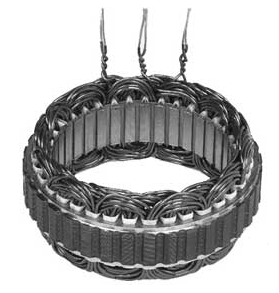
\includegraphics[scale=1]		{figuras/estator_alternador.png}
	\caption{Estator do alternador}
	\label{estator-alternador}
\end{figure}

\item [Conjunto Retificador]

A tensão e a corrente produzida no alternador são alternadas (justificativa para o nome alternador), conforme já salientado neste relatório. Entretanto, essa tensão não serve para alimentar as cargas elétricas do nosso projeto, uma vez que a bateria de armazenamento/excitação do rotor do alternador requer corrente contínua. Por esse motivo, a tensão alternada gerada deverá ser retificada ou filtrada, com o objetivo de prosseguirmos com a fonte geradora adotada.

Seguindo essa linha de pensamento, há no gerador um dispositivo conhecido como conjunto retificador ou placa de diodos, cujo desempenho consiste em transformar a corrente e a tensão alternadas em contínuas.

Continuando, o supracitado conjunto retificador presente em nosso alternador são equipados com diodos Zenner, os quais protegem os dispositivos elétricos contra as cargas de retorno, sendo montados com o intuito de bloquear possíveis correntes reversas.


\item [Regulador de Tensão]

Uma vez que a tensão alternada necessária à produção de corrente elétrica deve estar em conformidade com o sistema elétrico do alternador, a fim de não danificar todo o sistema, torna-se necessário a presença de um dispositivo que regule a tensão do mesmo. Esse dispositivo é o regulador.
O regulador de tensão do alternador é um dispositivo de proteção do mesmo. É utilizado com o objetivo de proteger os equipamentos que usam a energia gerada pelo alternador, ou seja, as cargas conectadas a ele. 

O modo de funcionamento deste dispositivo de proteção das cargas ocorre por meio do controle da tensão produzida, em qualquer regime de rotação do alternador, de modo a limitar a tensão para que não haja picos de corrente elétrica.

Neste raciocínio, a função principal do regulador de tensão do alternador consistirá em impedir que a bateria utilizada em nosso projeto sofra sobrecarga, pois os terminais de saída do alternador estarão ligados aos terminais da bateria.
\end{description}

\subsection{Bateria}

A presença de uma bateria em nosso circuito justifica-se por meio de três motivos:

\begin{enumerate}
	\item Necessidade de armazenar a energia elétrica oriunda da conversão eletromecânica supracitada;
	\item Necessidade de continuidade do fluxo de energia elétrica para atender as cargas quando o alternador não for capaz de fornecer a corrente elétrica necessária à alimentação do circuito em tela.
	\item Necessidade inicial de uma fonte de excitação do enrolamento de campo do rotor do alternador.
\end{enumerate}

Nesse sentido, para que isso ocorra, tem-se por necessário que a tensão disponibilizada no terminal do alternador aqui utilizado seja superior à tensão dos polos da bateria para que seja mantido o fluxo da corrente elétrica proveniente do alternador para a bateria. Caso contrário, a bateria não receberá a energia elétrica gerada no alternador. Nesse ponto, a fim de constatar se a bateria está sendo carregada, será alocado entre a mesma e o alternador um multímetro, posicionado na grandeza voltagem. 
Pois bem, voltando-se a atenção para o dimensionamento da bateria a ser utilizada em nosso projeto, informa-se que o primeiro passo consiste em escolher uma bateria que apresente tensão inferior à do alternador. Continuando, o próximo passo do dimensionamento da bateria requer que esta seja capaz de fornecer a corrente elétrica necessária à correta alimentação das cargas. 
Desse modo, com base na tensão terminal do alternador projetado e na corrente elétrica requisitada pelas cargas presentes no circuito elétrico em abordagem, dimensionou-se a bateria de nosso circuito (Figura \ref{bateria}). 

\begin{figure}[h]
	\centering
	%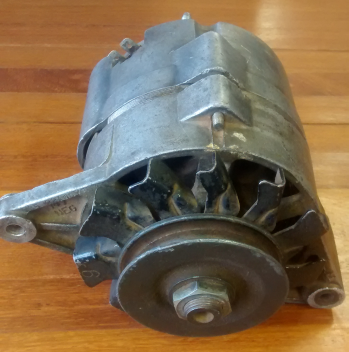
\includegraphics[scale=0.8]		{figuras/alternador.png}
	\caption{Imagem da bateria presente no Projeto Elétrico Start X}
	\label{bateria}
\end{figure}

Os dados nominais das grandezas elétricas pertinentes à bateria demonstrada na Figura acima foram listados na Tabela \ref{dados-bateria}.


\begin{table}[h]
\centering
\begin{tabular}{|l|l|}
\hline
\rowcolor[HTML]{329A9D} 
GRANDEZA ELÉTRICA                                                    & VALOR                                                   \\ \hline
Tensão& 12V 
\\ \hline
Corrente hora & 6Ah
\\ \hline
Potência hora  & 72Wh
\\ \hline
\end{tabular}
\caption{Dados nominais da bateria projetada.}
\label{dados-bateria}
\end{table}

Voltando-se a comentar a respeito da corrente de excitação do enrolamento de campo do rotor do alternador, foi dito acima que a literatura reporta a necessidade de 1\% da potência nominal do alternador para que o mesmo seja excitado e comece o processo de geração de energia elétrica baseando-se no princípio da indução eletromagnética. Pois bem, analisando-se as propriedades da Tabela anterior, verifica-se que a bateria aqui projetada atende à necessidade de potência informada acima, visto que 1\% da potência nominal do nosso alternador corresponde a 49 watts, sendo a potência da bateria igual a 72 watts hora, isto é, ela é capaz de fornecer durante 1 hora 72 watts mantendo sua tensão nominal.

\subsection{Dimensionamento dos Condutores}

O caminho percorrido pela energia elétrica ao longo de um circuito de distribuição deve ser projetado da maneira mais eficiente possível, desde a fonte geradora de corrente elétrica até as cargas terminais, uma vez que parcela daquela energia é dissipada sob a forma térmica devido à resistência elétrica que o fio condutor pelo qual a referida energia se movimenta exerce sobre o fluxo elétrico, restando, assim, prejudicada a eficiência final de distribuição da energia.

Nesse sentido, ao se projetar um circuito elétrico, deve-se procurar minimizar ao máximo possível as perdas de energia ao longo do mesmo e, agindo dessa maneira, por conseqüência, restaram observados aspectos ambientais e conservacionistas ligados ao desperdício de energia. Ademais, deve-se atentar que as perdas oriundas do calor gerado nos condutores de eletricidade reduzirão o nível da tensão disponível no circuito terminal.

Por isso, ao dimensionar os condutores pertinentes ao projeto elétrico ora em estudo, os aspectos acima mencionados foram levados em consideração, a fim de reduzir na prática as supracitadas perdas.
Seguindo esse raciocínio, a escolha dos condutores utilizados neste projeto foi realizada conforme algumas das especificações dispostas pela Associação Brasileira de Normas Técnicas (ABNT) na Norma Brasileira número 5410, de 2004 (NBR 5410:2004), cujo teor aborda critérios para o dimensionamento de instalações elétricas de baixa tensão.

Desse modo, cuidou-se em dimensionar os referidos condutores de acordo com os critérios que visam auxiliar economia de energia, bem como economia de custos financeiros, a fim de atender às necessidades do nosso projeto.

Assim, conforme especificações técnicas daquela NBR, cuidou-se em identificar a seção do condutor que reduza o custo da energia desperdiçada, sem incorrer em custos iniciais excessivos de compra e instalação de um cabo, bem como dos dispositivos de proteção necessários, pautando-se pelos seguintes métodos:

\begin{itemize}

	\item Capacidade de condução de corrente
	\item Queda de tensão
	\item Seção mínima
\end{itemize}

Ao final dos resultados, em princípio, cada um desses métodos poderá indicar uma seção diferente. Então, segundo a NBR, a seção a ser finalmente adotada consistirá na maior dentre todas as seções obtidas.

Desse modo, para que os métodos acima possam ser executados, inicialmente, torna-se necessário saber a corrente de projeto.

\subsubsection{Cálculo da Corrente de Projeto Necessária}

A corrente de projeto necessária ao atendimento das cargas a ser alimentadas pelo circuito de distribuição da energia elétrica gerada deve ser determinada conforme a Equação \ref{equacao-corrente}

\begin{equation}
	{I}_{proj} = \frac{{P}_{ativa}}{V \times FP}
	\label{equacao-corrente}
\end{equation}

Onde:
\begin{description}

\item [Iproj] corrente de projeto em ampère

\item [Pativa] potência ativa total do circuito em watt

\item [V] tensão do circuito em volt

\item [FP] fator de potência total do circuito
\end{description}

Nesse sentido, com base nos dados levantados para a potência requerida pelas cargas (32,5 W), na tensão nominal do alternador (14 V), e levando-se em consideração que as cargas são resistivas (fp = 1), tem-se que a corrente de projeto necessária será igual a aproximadamente 2,32 ampères.

Entretanto, a corrente de projeto a ser adotada para o dimensionamento dos condutores do circuito elétrico será tida como 35 ampères, devido ao fato deste valor ser a capacidade máxima de corrente elétrica que a fonte geradora aqui adotada poderá atingir.

O fato de a corrente de projeto ter sido escolhida acima da necessidade real de nosso projeto é justificado, ainda, pelo motivo da possibilidade futura de expansão das cargas alimentadas pelo circuito ora projetado, ocorrendo assim a desnecessidade de redimensionamento do sistema elétrico caso novas cargas fossem inseridas no mesmo.

\subsubsection{Capacidade de Condução de Corrente}

O dimensionamento do projeto elétrico seguindo todos os critérios mencionados na NBR em comento tem sua relevância, embora seja compreensível que o critério da capacidade de condução de corrente apresente uma importância que parece ser superior às demais, surgindo como ponto de partida da escolha dos condutores apropriados.

Ainda, o critério aqui discutido, de fato, logo após as determinações das cargas existentes no circuito e do cálculo da corrente de projeto (Iproj), pode ser considerado a primeiro passo em relação ao dimensionamento dos componentes do circuito, tendo como resultado a determinação da capacidade de condução de corrente do circuito, e por consequência, determinando assim a seção do condutor que proporcionará nas condições práticas de execução a capacidade de condução de corrente suficiente para a circulação de Iproj sem riscos.

Desse modo, em posse do valor de $I_{proj}$, bem como das características de constituição dos condutores, recorreu-se às tabelas que orientam o dimensionamento através do critério em análise, apurando-se a seção do condutor que atenda às necessidades do nosso circuito, vejamos.

Para o caso concreto, segundo as disposições da NBR, quanto ao tipo de condutor empregado, ter-se-á condutor isolado (condutor metálico e isolação), sendo o material PVC (cloreto de polivinila). Isso é devido às características de trabalho listadas na Tabela \ref{nbr}, com informações extraídas da NBR.

\begin{table}[h]
\centering
\begin{tabular}{| c | p{3cm} | p{3cm} | p{3cm} |}
\hline
\rowcolor[HTML]{329A9D} 
Tipo de isolação                & Temperatura máxima para serviço contínuo (condutor) & Temperatura limite de sobrecarga (condutor) & Temperatura limite de curto-circuito (condutor) \\ \hline
Cloreto de polivinila(PVC)      & 70                                                 & 100                                        & 160                                            \\ \hline
Borracha etileno-propileno(EPR) & 90                                                 & 130                                        & 250                                            \\ \hline
Polietileno-reticulado(XLPE)    & 90                                                 & 130                                        & 250                                           
\\ \hline
\end{tabular}
\caption{Tipos de Isolação dos Condutores e Características Operacionais}
\label{nbr}
\end{table}

Cumpre informar que o motivo da escolha dos condutores com tipo de isolação PVC foi feita devido esse condutor suportar adequadamente as condições de nosso projeto, além de ser de fácil aquisição.

No que tange ao método de instalação a ser utilizado, levou-se em consideração o fato de que este influencia a capacidade de troca térmica entre os condutores e o ambiente circundante, alterando a capacidade de condução de corrente dos condutores. Por isso, dentre os vários métodos disponíveis na NBR, procurou-se por um que se assemelhasse às condições de nosso projeto. Nesse sentido, optou-se pelo método de instalação B1, para condutor isolado. As demais descrições deste método são informadas na Figura \ref{metodos-condutores}. Convém informar que as informações expostas na referida Figura foram extraídas da supracitada NBR.

\begin{figure}[h]
	\centering
	%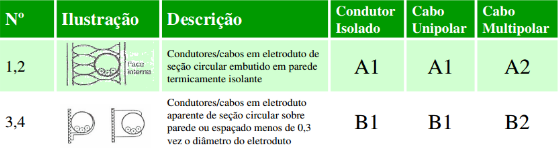
\includegraphics[scale=0.8]		{figuras/nbr.png}
	\caption{Alternativas para escolha do método de instalação dos condutores.}
	\label{metodos-condutores}
\end{figure}

 Continuando, a NBR diz que a Iproj adotada deve ser corrigida por fatores de correção apropriados, os quais são: a) fatores de correção para temperaturas ambientes diferentes; b) correção de resistividade do solo; e c) fator de correção de agrupamento. Uma vez que as condições de projeto do circuito em discussão não necessitam da utilização desses fatores, prosseguiu-se o dimensionamento com a Iproj anteriormente informada.
 
 O próximo passo foi determinar o esquema dos condutores, conforme opções listadas na Figura \ref{esquema-condutores}, também retiradas da supracomentada NBR. Optou-se pelo esquema monofásico a dois condutores.
 
 \begin{figure}[h]
	\centering
	%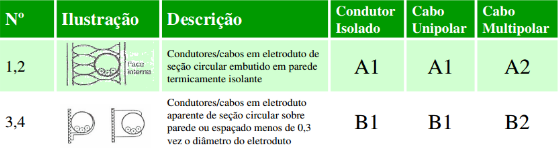
\includegraphics[scale=0.8]		{figuras/nbr.png}
	\caption{Determinação do esquema de condutores vivos do circuito.}
	\label{esquema-condutores}
\end{figure}

Após a definição dessas características/parâmetros, o próximo passo foi efetivar a escolha da seção dos condutores apropriados às condições de projeto. Assim, com base em dados disponibilizados pela Empresa Pirelli (Figura \ref{secao-condutores}), os quais são relacionados a dimensionamento de condutores consoante prescrições estipuladas na NBR 5410:2004, chegou-se à conclusão da seção nominal dos condutores de nosso projeto, conforme o método de capacidade de condução de corrente.

 \begin{figure}[h]
	\centering
	%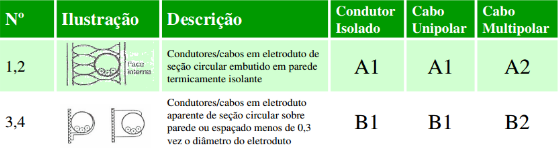
\includegraphics[scale=0.8]		{figuras/nbr.png}
	\caption{Determinação da seção dos condutores do Projeto Elétrico START X por meio do método da capacidade de condução de corrente.}
	\label{secao-condutores}
\end{figure}

Portanto, concluiu-se que a seção nominal dos condutores deverá ser igual à 6 mm\textsuperscript{2}.

\subsubsection{Queda de Tensão }

A importância da aplicação desse critério consiste no fato de que as cargas consumidoras de energia elétrica foram projetadas para trabalharem com determinado valor de tensão, aceitando, apenas, reduzida tolerância de não-conformidade com o valor de tensão nominal para o qual a carga foi projetada.

Assim, ao utilizar esse critério, foi levada em consideração a possibilidade dos efeitos anormais que a queda de tensão poderá acarretar às cargas.

 	Segundo esse critério, à medida que a distância entre o medidor de energia e a potência da carga aumenta a queda de tensão ao longo do condutor também aumenta. Por isso, baseando-se nessa justificativa, e com auxílio das características dos condutores adotados neste projeto (PVC, eletroduto não magnético e método de referência B1), somado ao fato de que a NBR informa que em baixa tensão a queda de tensão nos circuitos terminais não pode ser superior a 4\%, calculou-se a seção dos condutores, veja.
 	
\begin{description}

\item Cálculo da Queda de Tensão
	
	Para efetuar o cálculo da queda de tensão utilizou-se a Equação \ref{queda-tensao}.

\begin{equation}
	\Delta V = \Delta V_{\frac{V}{A \times km}} \times I_{proj} \times L
	\label{queda-tensao}
\end{equation}

Onde:

\begin{description}
	\item [$\Delta V$] percentual da queda de tensão admissível;
	\item [$\Delta V_{\frac{V}{A \times km}}$] queda de tensão em volt
	\item $I_{proj}$ corrente de projeto em ampère
	\item L comprimento do circuito em quilômetro
\end{description}

Nesse sentido, segue o memorial do cálculo em comento:

\begin{equation}
	\Delta V_{\frac{V}{A \times km}} = \frac{\Delta V} {I_{proj} \times L}
\end{equation}
\begin{equation}
	\Delta V_{\frac{V}{A \times km}} = \frac{0,04 \times 14}{35 \times 0,002}
\end{equation}
\begin{equation}
	\Delta V_{\frac{V}{A \times km}} = 8 \times \frac{V}{A \times km}
\end{equation}

\end{description}

Com esse resultado, visitou-se os dados disponibilizados pela Empresa Pirelli (Figura \ref{determinacao-secao}), os quais são relacionados a dimensionamento de condutores consoante prescrições estipuladas na NBR 5410:2004, chegando-se à conclusão da seção nominal dos condutores de nosso projeto, conforme o método da queda de tensão.

\begin{figure}[h]
	\centering
	%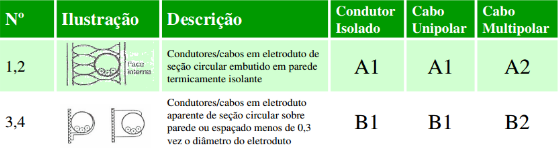
\includegraphics[scale=0.8]		{figuras/nbr.png}
	\caption{ Determinação da seção dos condutores do Projeto Elétrico START X por meio do método da queda de tensão.}
	\label{determinacao-secao}
\end{figure}

Nesse sentido, a seção dos condutores de nosso projeto deve ser igual a 4 mm\textsuperscript{2}.

\subsubsection{Seção Mínima}

As seções mínimas admitidas em qualquer instalação de baixa tensão estão indicadas na Figura \ref{secao-minima-condutores}, conforme disposições pertinentes ao método em cena, obtidas com arrimo na multicitada Norma 5410:2004, veja:

\begin{figure}[h]
	\centering
	%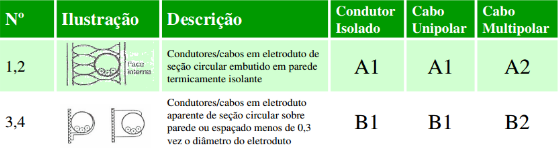
\includegraphics[scale=0.8]		{figuras/nbr.png}
	\caption{ Disposições a respeito do Método da Seção Mínima usado no dimensionamento dos condutores.}
	\label{secao-minima-condutores}
\end{figure}

Assim, dentro desse quesito, adotou-se que as ligações de nosso circuito serão do tipo flexíveis, sendo a utilização consistente com circuitos de extra-baixa tensão para aplicações especiais. Por isso, levando-se em consideração a Figura acima, a seção indicada é 0,75 mm\textsuperscript{2} para os condutores de cobre.
 	
 	Após realização dos três métodos (capacidade de condução de corrente, queda de tensão e seção mínima) chegou-se à conclusão de que a seção da bitola dos condutores do nosso circuito será de 6 mm\textsuperscript{2}, uma vez que é o maior resultado de seção obtido após cálculos baseados nos referidos métodos.
 	
\subsection{Dimensionamento dps Dispositivos de Proteção do Circuito}

A fim de manter o perfeito funcionamento do circuito ora em projeção, faz-se necessária a presença de dispositivos que o protejam contra condições adversas, isto é, condições acima das especificações nominais de operação dos elementos de circuito presentes no mesmo.
Em outras palavras, a função da mencionada proteção consiste justamente em minimizar os danos ao sistema e seus componentes, sempre que ocorrer uma falha no equipamento, no sistema elétrico ou ainda falha humana. Por isso, a escolha, a aplicação e a coordenação seletiva adequada ao conjunto de componentes que constituem a proteção de um projeto elétrico é um dos aspectos de suma importância.

Continuando, os dispositivos de proteção agem de maneira automática, sendo essa ação provocada por dispositivos sensíveis a determinadas condições anormais, no sentido de evitar ou limitar danos a um sistema ou equipamento, conforme já salientado, resguardando-o dos possíveis efeitos adversos, como por exemplo, uma sobrecarga ou curto-circuito.

Nesse passo, para o nosso projeto, os dispositivos de proteção utilizados consistirão em fusíveis de vidro (Figura \ref{fusivel}), além do regulador de tensão e dos diodos Zenner já presentes na estrutura do alternador.

\begin{figure}[h]
	\centering
	%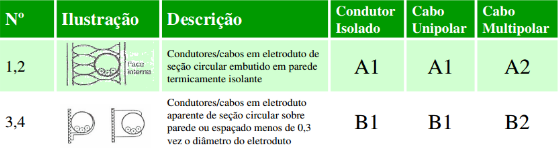
\includegraphics[scale=0.8]		{figuras/nbr.png}
	\caption{Imagem do fusível de vidro utilizado no Projeto Elétrico Start X.}
	\label{fusivel}
\end{figure}

Os fusíveis são dispositivos de segurança cuja função é interromper o fluxo de corrente elétrica no ramo do circuito considerado quando a corrente ultrapassar a especificação nominal dele, evitando-se, assim, um curto-circuito. Ainda, esses dispositivos protegem qualquer tipo de carga, tanto reativa, (picos de correntes que podem ocorrer nessas cargas) quanto resistiva (onde a variação de corrente não é grande, funcionando como prevenção).

Nesse sentido, chega-se, então, aos motivos que nos levaram a optar pelos fusíveis, dentre outras explicações, citando-se o baixo custo de aquisição dos mesmos, bem como devido ao seu modo de operação ser bastante simples. 

Assim, para o dimensionamento dos fusíveis aqui utilizados foram observadas três características fundamentais, as quais especificam o modo de operação dos mesmos: corrente nominal, corrente de curto-circuito e tensão nominal. 

As referidas características foram levantadas de acordo com as características das cargas e condições dos ramos dos circuitos que serão protegidos pelos fusíveis, a fim destes funcionarem adequadamente no tocante à proteção das cargas. Portanto, com base nessas informações, chegou-se a conclusão que os fusíveis requeridos ao nosso circuito deverão ser conforme as especificações dispostas na Tabela \ref{propriedade-fusivel}.
 	
\begin{table}[h]
\centering
\begin{tabular}{|l|l|}
\hline
\rowcolor[HTML]{329A9D} 
GRANDEZA  & VALOR                                                   \\ \hline
Corrente Nominal(A) & 0,98 
\\ \hline
Corrente de Curto-Circuito(A) & 1
\\ \hline
Tensão Nominal(V)  & 250
\\ \hline
\end{tabular}
\caption{Propriedades nominais dos fusíveis utilizados no Projeto Start X.}
\label{propriedade-fusivel}
\end{table}

\subsection{Dimensionamento de eletroduto}

Também conhecido como conduíte, o eletroduto é o elemento que protege os condutores elétricos contra influências externas, como choques mecânicos e agentes químicos. Têm, ainda, a função de controle de chamas em caso de incêndio provocado por curto-circuito. 
A figura \ref{eletrodutos} mostra os tipos de eletrodutos.

\begin{figure}[h]
	\centering
	%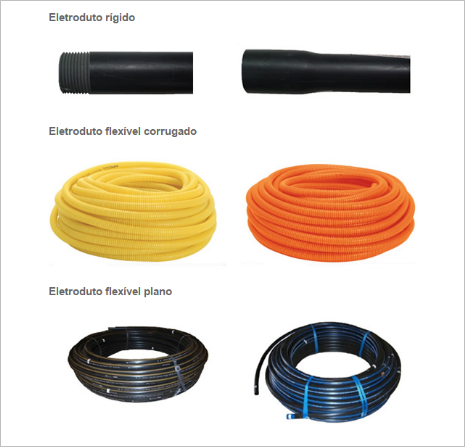
\includegraphics[scale=0.8]		{figuras/eletrodutos.png}
	\caption{Tipos de Eletrodutos}
	\label{eletrodutos}
\end{figure}

\subsubsection{Especificação}

Entre as características que precisam de atenção está a verificação da curvatura. Ou seja, após ser submetido a uma determinada sequência de dobramentos, o produto tem que permitir a passagem da fiação sem problemas ou obstruções. A resistência à compressão e a impactos também deve ser observada.

Os eletrodutos são fabricados para resistirem ao calor e ao fogo. Nos ensaios realizados em laboratórios, têm que suportar 60ºC durante 24 horas sem apresentar qualquer deformidade. Seu desempenho elétrico também é testado, sendo que não devem permitir a passagem de corrente com valores superiores a 100mA e a resistência elétrica deve ser inferior a 100M$\Omega$.

A versão corrugada amarela é específica para aplicações leves e, normalmente, instalada embutida em parede. Já a laranja, também corrugada, é para aplicação em lajes, onde a exigência por resistência aos esforços mecânicos é maior. Os rígidos, produzidos na cor preta, são ainda mais resistentes aos esforços mecânicos que podem ocorrer durante a concretagem da laje. A principal diferença entre eles está na resistência diametral.

\subsubsection{Aplicação}

O uso do eletroduto é definido de acordo com sua resistência mecânica (leve, médio ou pesado), e com a classificação quanto à propagação de chama. A instalação dos produtos deve seguir a ABNT NBR 5410:2004 – Instalações Elétricas de Baixa Tensão –, que especifica as condições a que devem satisfazer as instalações elétricas de baixa tensão de edificações

\subsubsection{Vantagens}

O gerente do produto certo para cada aplicação, além do respeito às normas técnicas, para garantir um executivo comenta que o custo-benefício está diretamente ligado à escolha desempenho satisfatório.  Os conduítes são materiais facilmente encontrados no mercado, visto que qualquer revenda especializada em elétrica deve dispor, no mínimo, das três versões mais comuns do material.

\subsubsection{Dimensionamento}
Dimensionar um eletroduto é determinar o tamanho nominal do eletroduto para cada trecho da instalação.

O tamanho nominal do eletroduto é o diâmetro externo do eletroduto, este tamanho é expresso em milímetros(mm) é e padronizado pela norma NBR 5410:2004.

Segundo a norma NBR 5410:2004 o tamanho dos eletrodutos deve ser de um diâmetro tal que os condutores possam ser facilmente instalados ou retirados. Por isso a norma estabelece que o eletrodutos tenha um diâmetro 60\% maior que os condutores, ou seja, é obrigatório que os condutores não ocupem mais que 40\% da área útil dos eletrodutos. A figura \ref{tamanhos-eletrodutos} demostra como isso pode mensurado de maneira simples.[2]

\begin{figure}[h]
	\centering
	%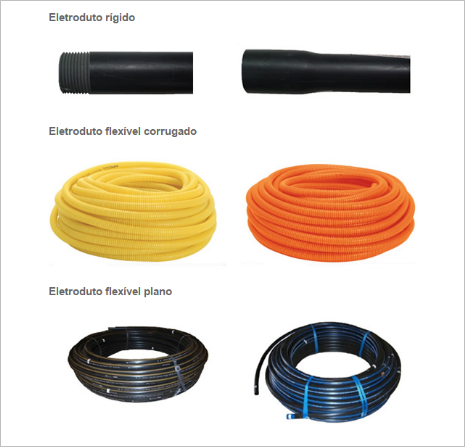
\includegraphics[scale=0.8]		{figuras/eletrodutos.png}
	\caption{Tamanhos de eletrodutos}
	\label{tamanhos-eletrodutos}
\end{figure}

Para melhor explicação a norma afirma que uma das formas de dimensionamento dos eletrodutos segue o seguinte roteiro:

\begin{enumerate}

	\item Determinar a seção dos condutores que irão passar no interior do eletroduto
	\item Determinar a area total de cada condutor, lembrando de considerar a camada de isolação de cada um.
	\item Efetuar a somatoria das seçoes totais dos condutores a serem utilizados.
	\item Em uma instalação eletrica o eletroduto deve ter um diamentro minimo de 20mm estes eletrodutos não são cotados na planta, este caso se refere a instalações prediais.
\end{enumerate}

A norma mostra que outra forma de dimensionar o eletroduto é em função da quantidade de condutores e a seção nominal do maior condutor no eletroduto. 

A ABNT NBR 5410:2004 admite, em 6.2.10.2, que os condutos fechados em geral e os eletrodutos em particular contenham condutores de mais de um circuito se as seções nominais dos condutores de fase estiverem contidas dentro de um intervalo de três valores normalizados sucessivos, tais como 1,5, 2,5 e 4 mm\textsuperscript{2}, 6, 10 e 16 mm\textsuperscript{2} ou 35, 50 e 70 mm\textsuperscript{2}, e assim por diante. Dessa forma, por exemplo, pode-se colocar dentro de um eletroduto cabos com seções de 1,5, 2,5 e 4 mm\textsuperscript{2}, mas não se podem colocar juntos num eletroduto cabos com seções de 1,5, 6 e 10 mm\textsuperscript{2}.

Em 6.2.11.1.6, determina-se a quantidade máxima de condutores dentro de um eletroduto, de modo a se deixar uma boa área livre no interior do eletroduto para facilitar a dissipação do calor gerado pelos condutores e facilitar a enfiação e retirada dos cabos. Para tanto, é necessário que os condutores ou cabos não ocupem uma porcentagem da área útil do eletroduto superior a 53\% para um condutor, 31\% para dois condutores e 40\% para três ou mais condutores.

Com base nessa prescrição, a maneira de calcular a quantidade máxima de condutores é resumida em comparar a área interna de um eletroduto com a área total de condutores. Da geometria, a área útil de um eletroduto (AE) é dada por:

\begin{equation}
	A_e = \frac{\pi}{4} \times \left(de - 2e\right) ^ 2
\end{equation}

Em que: de é o diâmetro externo do eletroduto e e a espessura da parede do eletroduto. Tais valores podem ser obtidos no catálogo do fabricante.
 

A área total de um cabo isolado (Ac) deve ser calculada por:

\begin{equation}
	A_c = \frac{\pi \times d ^ 2}{4}
\end{equation}

Sendo: d o diâmetro externo do cabo isolado, valor que é obtido no catálogo do fabricante.

Dessa forma, o número máximo (N) de cabos isolados, de mesma seção, que pode ser instalado em um eletroduto, é dado por:

\begin{equation}
	N = \frac{toc \times A_e}{A_c}
\end{equation}

Em que: toc = 0,53 para um condutor, 0,31 para dois condutores e 0,40 para três ou mais condutores a serem instalados no interior do eletroduto.

Para o trabalho em questão o grupo optou por utilizar o eletroduto flexível o eletroduto escolhido pelo grupo, segundo os cálculos foi o de 16 mm de diâmetro da marca TIGRE corrugando flexível como pode ser observado na figura \ref{eletroduto-tigre}

\begin{figure}[h]
	\centering
	%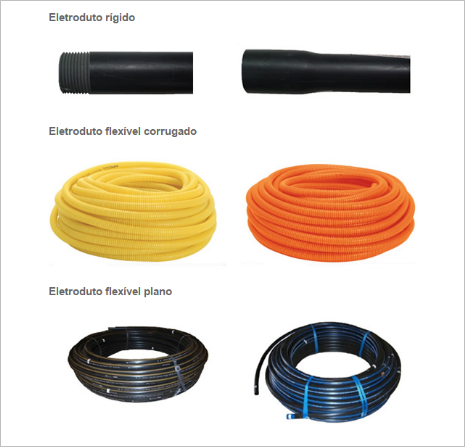
\includegraphics[scale=0.8]		{figuras/eletrodutos.png}
	\caption{Eletroduto marca TIGRE}
	\label{eletroduto-tigre}
\end{figure}

\subsection{Dimensionamento dos Circuitos de Alimentação das Cargas}

Os circuitos de alimentação das cargas referente ao Projeto Elétrico Start X consistirão em dois ramos a partir da bateria, sendo um deles destinado à alimentação dos sensores, enquanto o outro será destinado à alimentação do carregador de celular. Pois bem, passemos a discutir a respeito dos detalhes dos mesmos.

Na saída da bateria, a tensão aplicada às cargas pode apresentar-se com ondulação bastante acentuada, não desejada para a aplicação no circuito eletrônico dos sensores utilizados em nosso projeto. Deste modo, para que a tensão de saída da bateria ou tensão de entrada das cargas se torne mais uniforme possível, faz-se necessário o uso de algum tipo de filtro. O filtro mais utilizado é o filtro capacitivo, cujo objetivo reside na redução da ondulação da tensão de saída da bateria. Assim, serão utilizados filtros desse modelo em nosso circuito.

Além do filtro capacitivo, estarão presentes nos ramos dos circuitos dispositivos reguladores de tensão. O objetivo desses reguladores em nosso projeto consiste em adequar a tensão de saída da bateria (12 V) à tensão requerida pelas cargas aqui presentes. Nesse sentido, usar-se-ão reguladores de tensão na forma de circuitos integrados de três terminais, mais adequado ao nosso projeto, devido termos baixa potência no mesmo.

Continuando, no ramo de alimentação dos sensores será empregado um regulador de tensão da série 7805, o qual será antecedido pelos supramencionados capacitores que, por sua vez, são antecedidos pelo fusível já dimensionado. Esse ramo de alimentação apresentado na Figura \ref{fonte-reguladora}, juntamente com o fusível utilizado. 

\begin{figure}[h]
	\centering
	%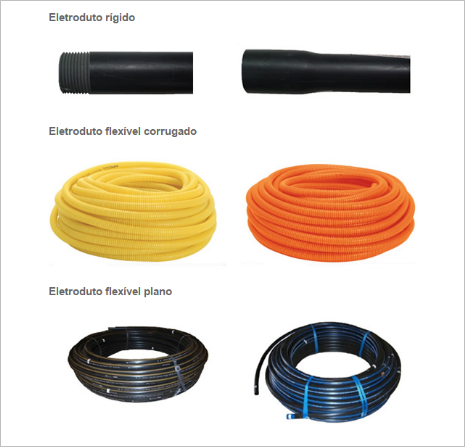
\includegraphics[scale=0.8]		{figuras/eletrodutos.png}
	\caption{Dispositivos elétricos presentes em dos ramos do circuito do Projeto Elétrico Start X. }
	\label{fonte-reguladora}
\end{figure}

O regulador de tensão da série 7805 foi escolhido devido este apresentar-se adequado às grandezas elétricas nominais dos sensores de nosso projeto, visto que aquele regulador de tensão regula tensões de entrada de até 35 volts (aqui, a tensão de entrada no mesmo consiste em 12 V, proveniente da bateria). Convém informar que, para o correto funcionamento do mencionado regulador de tensão, a tensão de entrada do mesmo dever ser no mínimo 2 volts mais alta que a tensão desejada na saída. Desse modo, como a tensão de saída no regulador de tensão em apreço deverá ser igual à tensão de entrada dos nossos sensores (5 V), resta atendido essa informação. Ainda em relação à justificativa de adoção do regulador de tensão aqui referenciado, informa-se que o mesmo tem tensão positiva com corrente de até 1 ampère de saída (o conjunto de sensores requer 500 mA).

Com relação aos filtros capacitivos empregados em nosso projeto, utilizar-se logo após o fusível dimensionado um capacitor eletrolítico de 100 micro-ampères, cuja finalidade é filtrar a frequência de entrada de modo a não permitir que entre no ramo de alimentação das cargas nenhuma tensão com frequência maior do que a desejada em nosso projeto. Ainda, após esse primeiro filtro capacitivo, será empregado um capacitor de poliéster de 100 nano-ampères, A finalidade dele consiste em filtrar a saída para que não passem frequências baixas.

Pois bem, com o intuito de se constatar a fidedignidade dos valores nominais inerentes aos filtros capacitivos, bem como do regulador de tensão 7805 empregados no ramo de alimentação dos sensores, realizou-se um teste em laboratório. O resultado prático desse teste encontra-se demonstrado na Figura \ref{teste-pratico}.

\begin{figure}[h]
	\centering
	%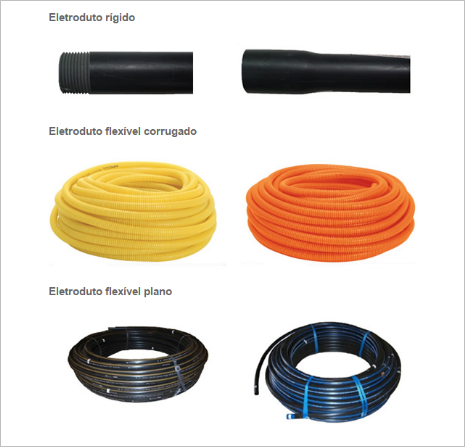
\includegraphics[scale=0.8]		{figuras/eletrodutos.png}
	\caption{Imagem do teste prático demonstrado a tensão de saída da bateria ao passar por fusível, filtros capacitivos e regulador de tensão da série 7805.}
	\label{teste-pratico}
\end{figure}

Como o único objetivo do sistema de geração de energia não é apenas fornecer energia elétrica para a alimentação dos sensores mas também para pequenas cargas foi feito em paralelo ao circuito de alimentação de 5 volts um circuito de alimentação variável para que uma gama maior de equipamentos e dispositivos possam ser ligados ao sistema. O regulador de tensão variável usa um potenciômetro que pode regulado para fazer que essa parte do circuito atenda atenções de 2,3 a 12,63 volts. A figura \ref{circuito-alimentacao} mostra o circuito feito pelo grupo com os dois reguladores de tensão.

\begin{figure}[h]
	\centering
	%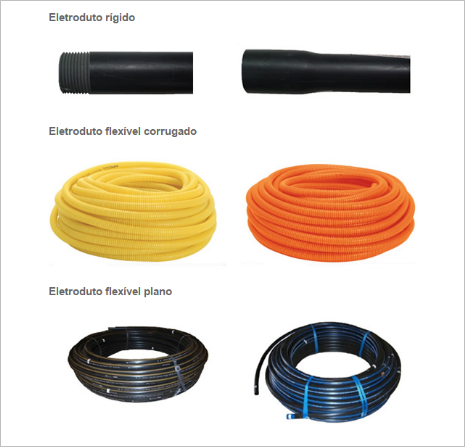
\includegraphics[scale=0.8]		{figuras/eletrodutos.png}
	\caption{Circuitos de alimentação constante (5V) e variável. }
	\label{circuito-alimentacao}
\end{figure}

\subsection{Representação Esquemática do Circuito  de Armazenamento/Distribuição do Projeto Elétrico Start X}

Depois de explicado e detalhado o funcionamento dos dispositivos elétricos e eletrônicos presentes em nosso projeto, apresenta-se a seguir o esquema pertinente ao circuito de armazenamento e distribuição de energia elétrica referente o Projeto Start X. 

\begin{figure}[h]
	\centering
	%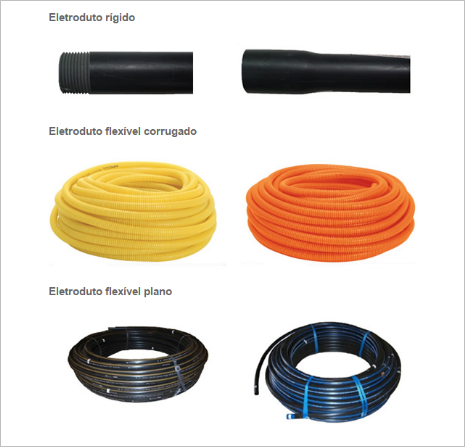
\includegraphics[scale=0.8]		{figuras/eletrodutos.png}
	\caption{Esquema do circuito}
	\label{ciruito}
\end{figure}
